\section{Introduction}


\subsubsection{Background}
Systems such as neurons can have different types of input. The authors\supercite{Smyth:1996} propose dividing the input to a neuron into receptive (or driving) and contextual. They further present formulations of how contextual connections can modulate driving input. Finally, they use information theory to compare and contrast contextual modulation in these different formulations.

\subsubsection{Motivation}
This work was published in 1996, but with the advances in computing and information theory, and increased emphasis on the importance of context\supercite{Larkum:2013}, new studies\supercite{Kay:2011,Wibral:2017} have started building on its foundations. Furthermore, there are many ways to write the activation functions and only a few simple formulations were analyzed. Therefore, the significance of this work is twofold: 1. To replicate the study in a modern programming language and make it publicly accessible.   2. Enable new activation functions to be readily tested.

\subsubsection{Replication}
A successful attempt is made to qualitatively and quantitatively replicate the results of the original paper by replicating the three figures that comprise the results. While in all cases the results are qualitatively identical, there are minor quantitative differences in some figures which could in some cases be attributed to the use of a different seed value or the differences between how small or large values are handled in this python implementation and the original authors' implementation in an old programming environment about three decades ago. 

\section{Methods}


\subsubsection{Input}
The study is limited to information transmission from a neuron which has only one receptive (R) or contextual (C) connection as input and produces one output (X). There is input at every time step, +1 denotes firing and -1 being silent, which is then multiplied by the weight of their connection. Probability distributions were created in the same way as original authors as described below, where for all figures P(C = 1 | R = 1) was set to 0.889972. This is so that the three components had all the same maximum possible value (0.5 bits). This makes it easier to compare the absolute values. 

\begin{equation}
P(R = +1, C = +1) = 0.5P(C = 1 | R = 1)
\end{equation}

\begin{equation}
P(R =+1, C = -1) = 0.5[1 - P(C = 1 | R = 1)]
\end{equation}

\begin{equation}
P(R = -1, C = +1) = 0.5[1 - P(C = 1 | R = 1)]
\end{equation}

\begin{equation}
P(R = -1, C = -1) = 0.5P(C = 1 | R = 1).
\end{equation}


\subsubsection{Activation Functions}
Three activation functions are studied by the authors. Based on how receptive and contextual information are formulated to interact, they are called A\textsubscript{a} (additive), A\textsubscript{m} (modulatory), and A\textsubscript{b} (both additive and modulatory). 

\begin{equation}
A_a(r,c) = r + c 
\end{equation}

\begin{equation}
A_m(r,c) = 0.5r[1 + e^{rc}] 
\end{equation}

\begin{equation}
A_b(r,c) = 0.5r[1 + e^{rc}] + c  
\end{equation}


Where r is an instance of  R, and c an instance of C, multiplied by the weight of the connection. The output of each activation function is passed into the sigmoidal activation function to generate a probability of firing:

\begin{equation}
p(X=1 | r,c) = \frac{1}{1 + e^{-A(r,c)}} 
\end{equation}


\subsubsection{Information Theory}
They use the three-way mutual information as a measure of the information shared between the output and the inputs which is defined as follows:

\begin{equation}
I(X;R;C) = \sum_{x,r,c}p(x,r,c)log\frac{P(x|r)P(x|c)}{P(x)P(x|r,c)}
\end{equation}

I(X;R|C) is used by the authors as a measure of information that is shared between the R input and the X output but not the C input and is defined as follows: 

\begin{equation}
I(X;R|C) = \sum_{x,r,c}P(x,r,c)log\frac{P(x|r,c)}{P(x|c)}
\end{equation}

I(X;C|R) is used by the authors as a measure of information that is shared between the C input and the X output but not the R input and is defined as follows:

\begin{equation}
I(X;C|R) = \sum_{x,r,c}P(x,r,c)log\frac{P(x|r,c)}{P(x|r)}
\end{equation}


\subsubsection{Dependencies} The replication was done using Ubuntu 19.10 with Intel® Core™ i7-7500U CPU with Anaconda Python-3.8.1, numpy-1.18.1, scipy-1.4.1, and matplotlib-3.1.3. There are no external libraries required for calculating the information theoretic terms as everything is provided in the accompanying code.

\section{Results}


\subsubsection{Activation functions and transmitted information}

Figure 1 shows the three-way mutual information and conditional mutual information terms for each of the activation functions and across a range of R input weights while C remains constant at 1. These results are produced in a similar way to the paper by using the exact probability distributions. They are qualitatively identical to the original paper. There are minor quantitative differences. For example, in (c) the maximum value of the $A_b$ function is higher in the original paper.  In order to rule out the possibility of missing the higher maximum value due to not having that particular data point, a step size of 0.1 was used for each data point which leads to a higher number of data points on this figure than the original publication's. 

\begin{figure}[H]
    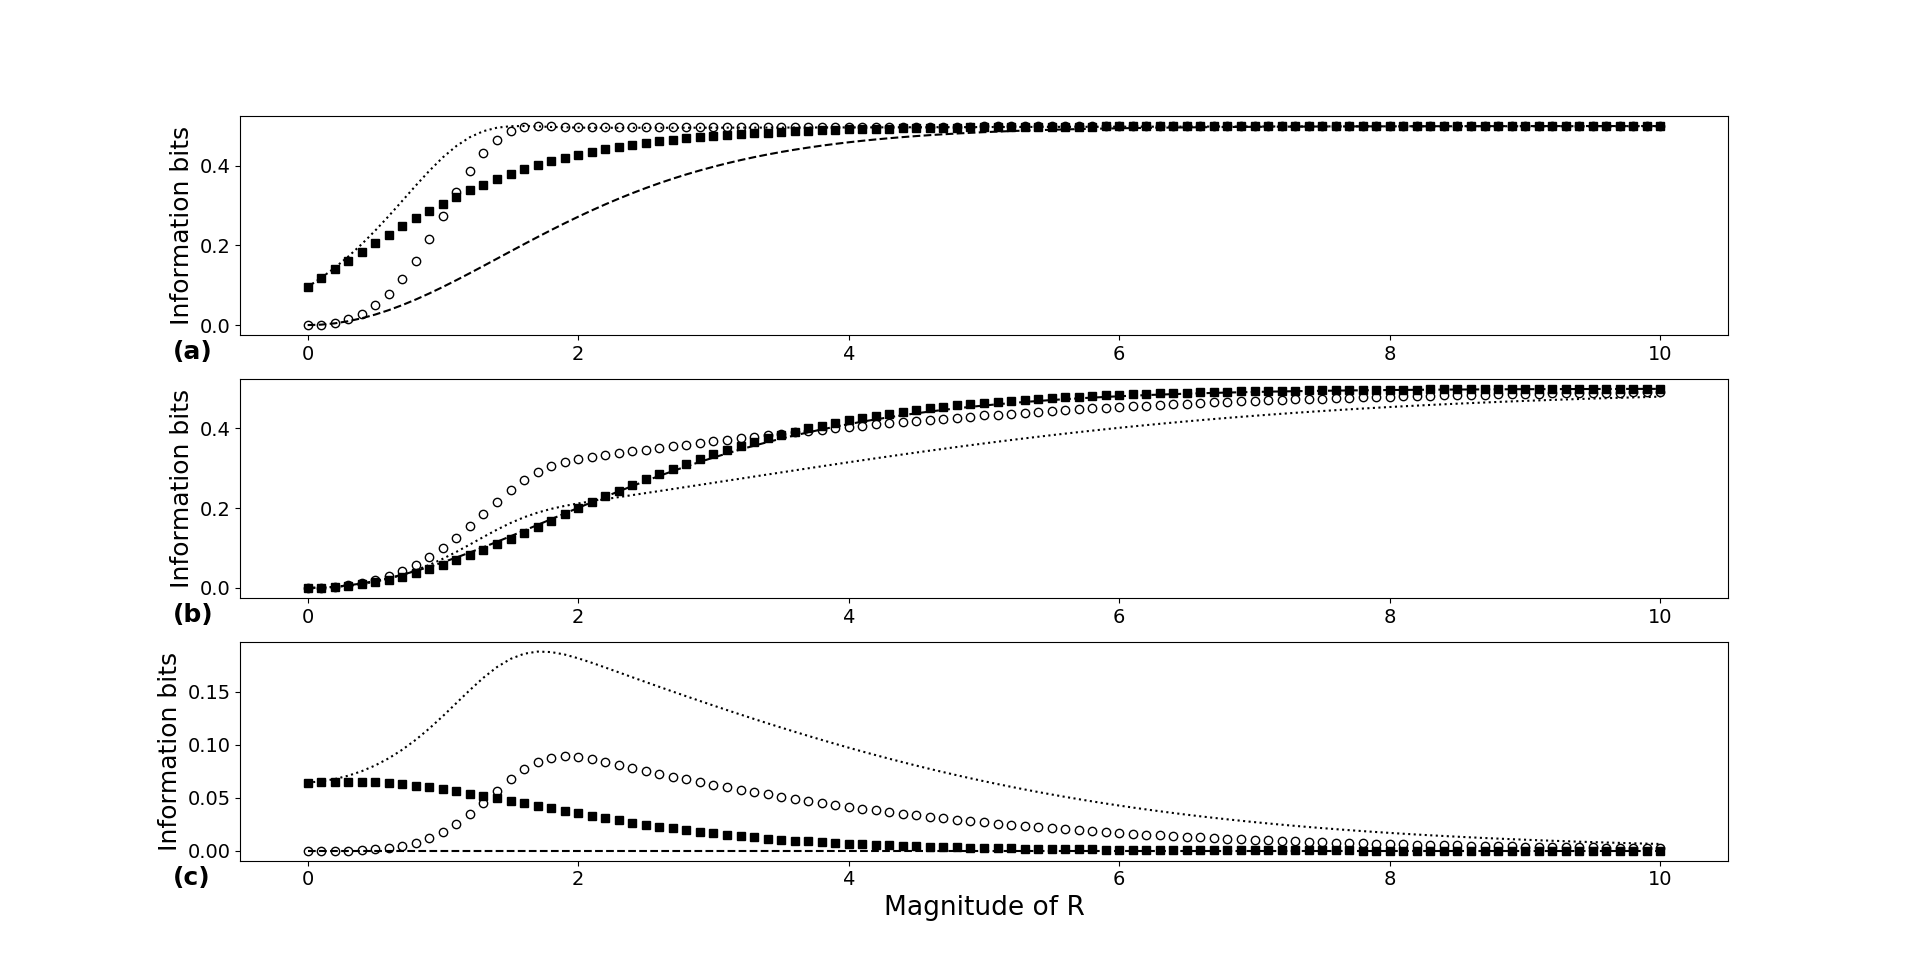
\includegraphics[width=\textwidth]{figure_1.png}
      \caption{Replication of the comparison of the activation functions for (a) I(X;R;C), (b) I(X;R|C) and (c) I(X;C|R). The activation functions are zero context (dashed), additive context (squares), modulatory context (circles), and both additive and modulatory combined (dotted).}
\end{figure}

\subsubsection{Information surface plots for different input weights}

Figure 2 shows the I(X;C|R) for each of the activation functions and across a range of r and c input weights. These results are produced in a similar way to the paper by using the exact probability distributions. They are qualitatively identical to the original paper. There are no notable quantitative differences. 


\begin{figure}[H]
    \begin{center}
        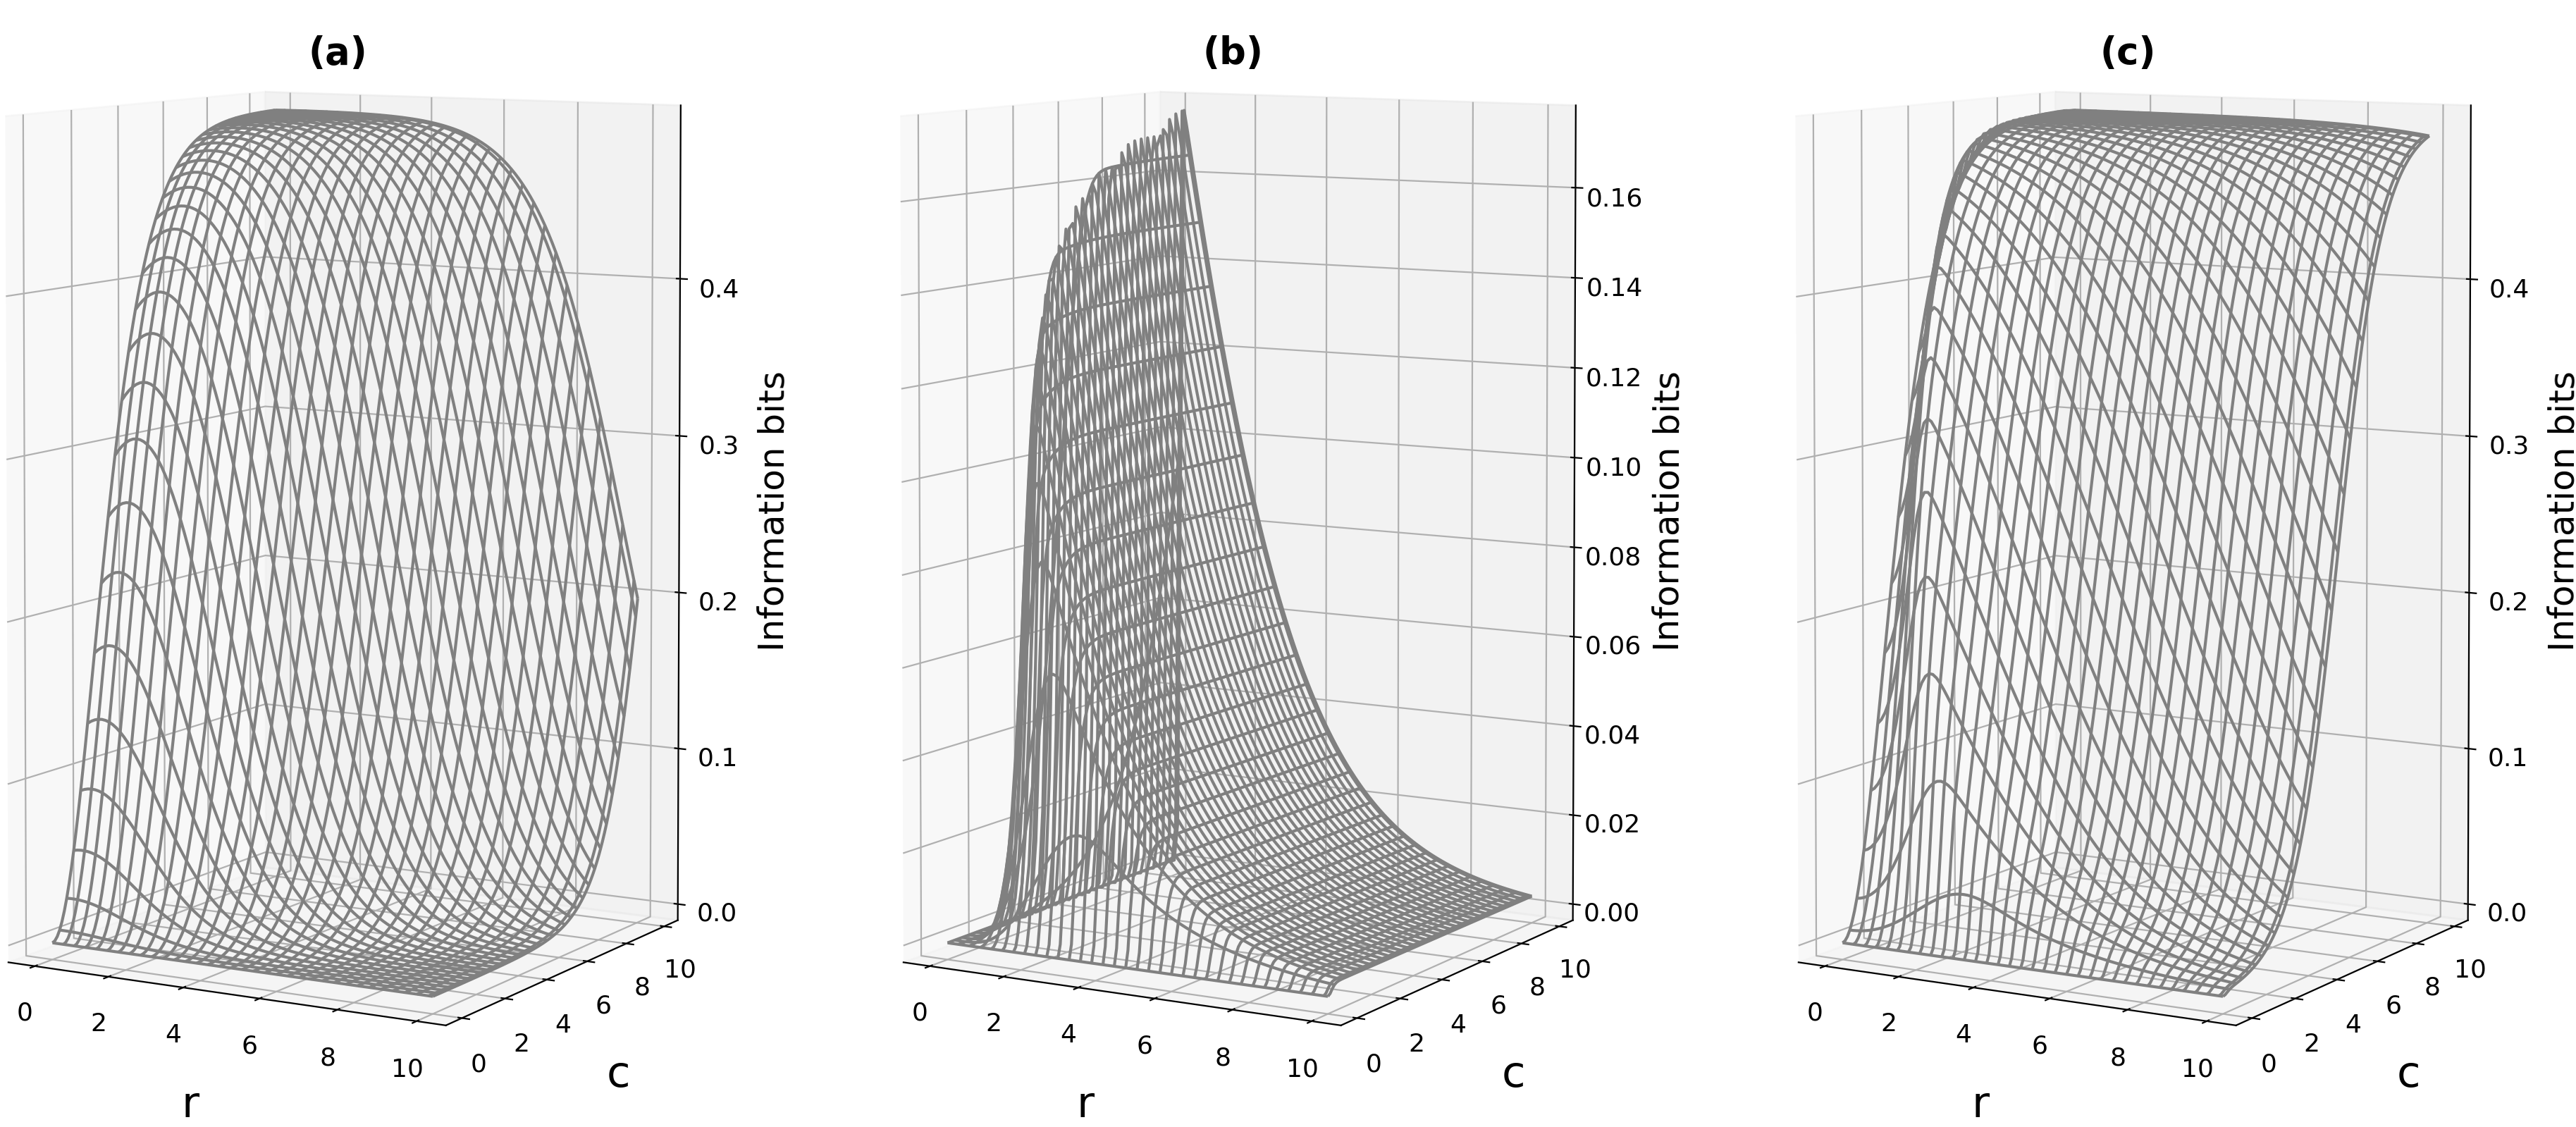
\includegraphics[width=12cm,height=15cm]{figure_2.png}
    \end{center}
      \caption{Replication of the comparison of the information surfaces of I(X;C|R) for (a) additive, (b) modulatory and (c) both over all R and C input weights. The conditional probability P(C = 1 |R = 1) = 0.889972.}
\end{figure}

\subsubsection{Sampling biases and variances}

Figure 3 compares the mean and standard deviation of three-way measures sampled against the analytical measures for the modulatory activation function. The mean and deviations were computed from 100 trials per sample size and compared with the analytical measure across a range of sample sizes. As the authors claim, sample size of 200 could be sufficient as the improvements beyond that are not much. The error for small sample sizes is higher in the original paper, this can be attributed to use of a different seed value and their programming environment.


\begin{figure}[H]
    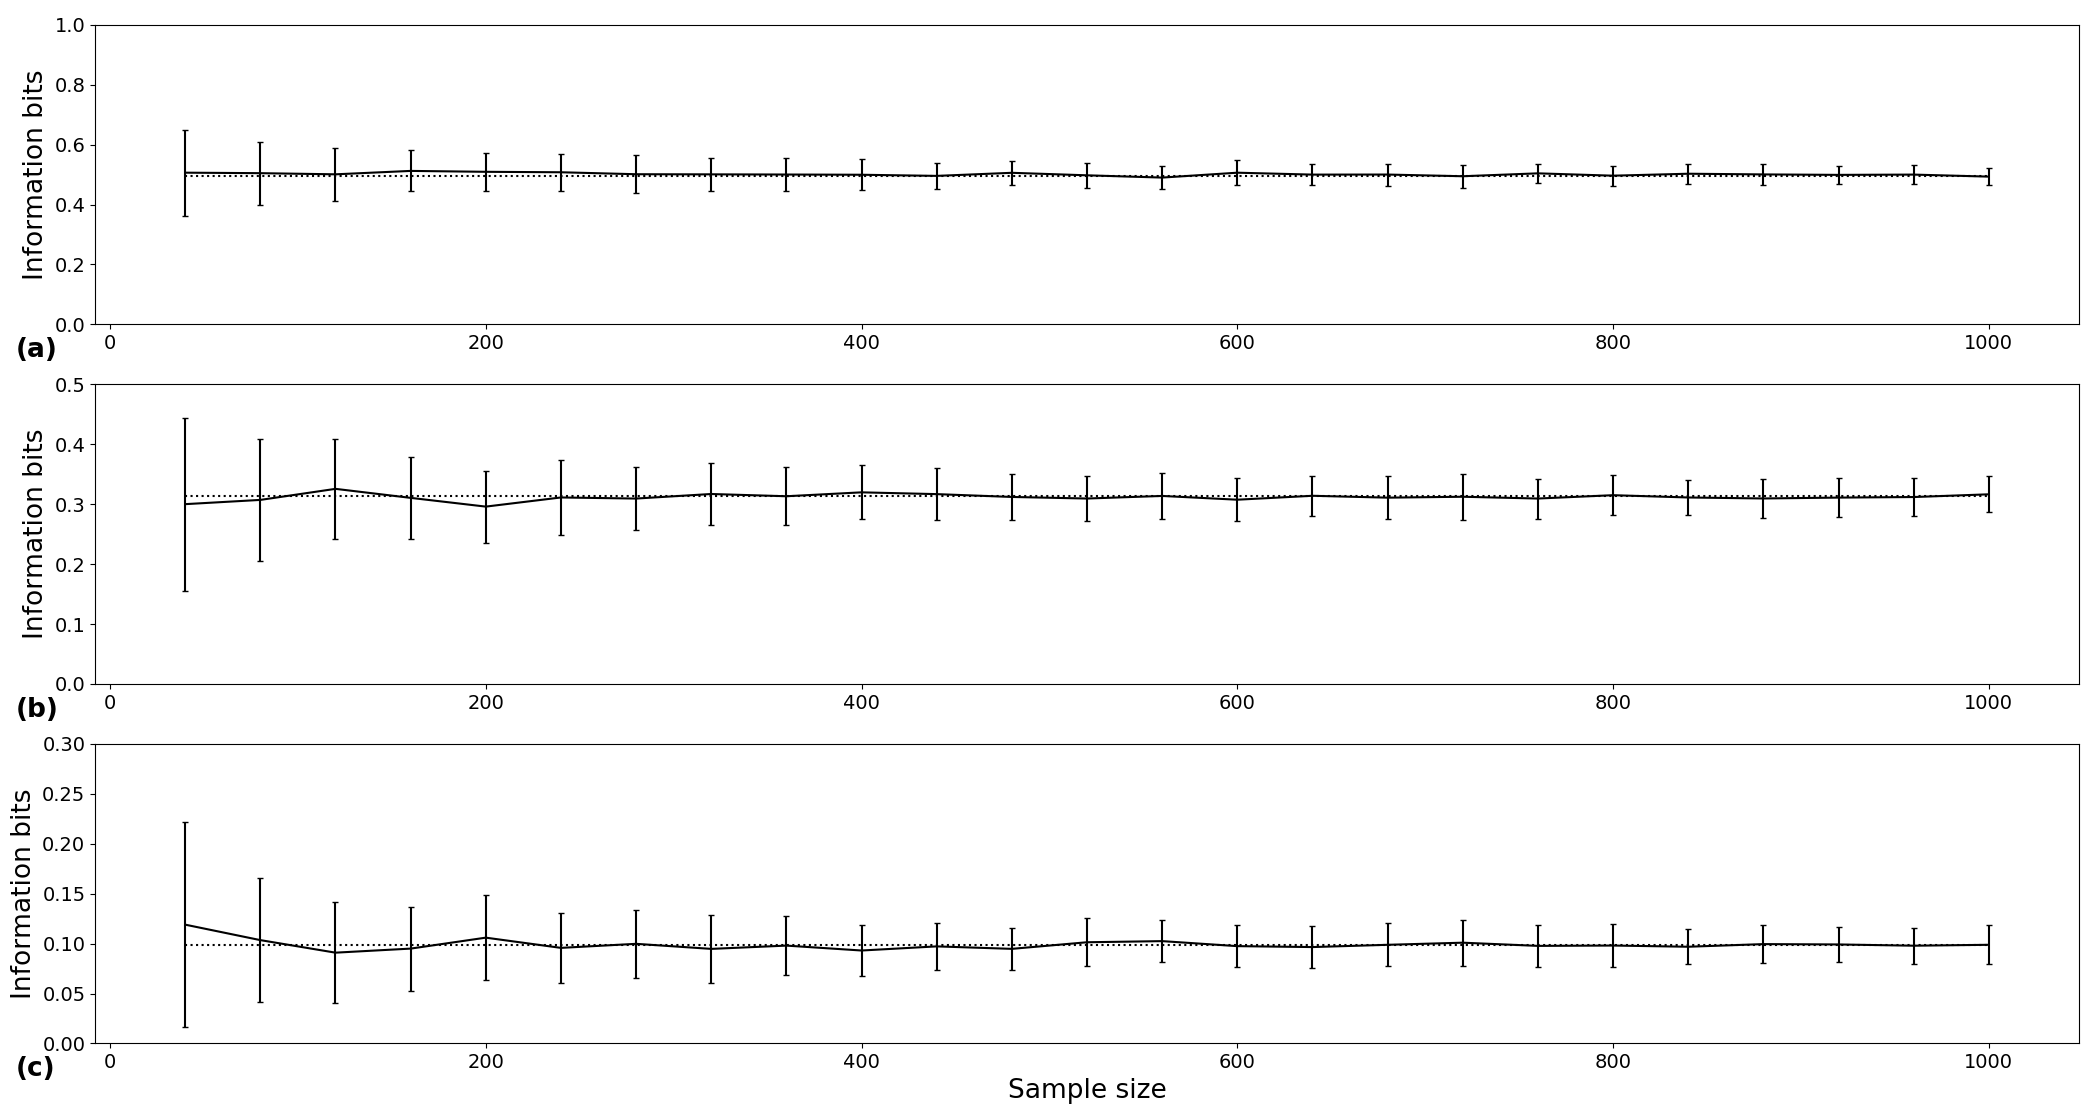
\includegraphics[width=\textwidth]{figure_3.png}
      \caption{Replication of comparison of the analytical (dotted) and sampled (error bars) information measures for (a) I(X;R;C), (b) I(X;R|C) and (c) I(X;C|R). The error bars represent standard deviation about the mean information computed from 100 trials for each sample size with the modulatory activation function. The R and C input weights were set to 2.}
\end{figure}

\section{Discussion}

The goal of the authors was to study contextual modulation in single binary neurons using information theory. To that end they present figures 1-2 as a way to compare and contrast functions with or without forms of contextual modulation. They use figure 3 to suggest how much data is required to get the required accuracy for the analyses presented in figures 1-2. \newline

One example of how the analyses here can be used to study contextual modulation is included as follows: For the modulatory activation function, it is intended that the role of R is to drive the neuron to fire and C is to amplify the firing. Figure 2 (b) shows that increasing C alone does not increase I(X;C|R), but increasing R and C together does and a higher C with a constant R amplifies it. At low R values, C has a higher role in the output so I(X;C|R) begins to diminish at higher R values. This shows that the modulatory function is behaving as intended and expected. \newline

In conclusion, this manuscript and the accompanying code present a successful replication of the authors' work in a modern programming language. Similarly, the code and information-theoretic analyses here could be used to study other activation functions and contextual modulation.

\subsubsection{Acknowledgments}

I would like to thank Bill Phillips and Jim Kay for clarifying my questions about the input. This research was supported by the funding initiative Niedersächsisches Vorab of the Volkswagen Foundation and the Ministry of Science and Culture of Lower Saxony.
